\documentclass[notes,11pt, aspectratio=169]{beamer}

\usepackage{pgfpages}
% These slides also contain speaker notes. You can print just the slides,
% just the notes, or both, depending on the setting below. Comment out the want
% you want.
\setbeameroption{hide notes} % Only slide
%\setbeameroption{show only notes} % Only notes
%\setbeameroption{show notes on second screen=right} % Both

\usepackage{helvet}
\usepackage[default]{lato}
\usepackage{array}
\usepackage{tgbonum}

\usepackage{tikz}
\usepackage{verbatim}
\setbeamertemplate{note page}{\pagecolor{yellow!5}\insertnote}
\usetikzlibrary{positioning}
\usetikzlibrary{snakes}
\usetikzlibrary{calc}
\usetikzlibrary{arrows}
\usetikzlibrary{decorations.markings}
\usetikzlibrary{shapes.misc}
\usetikzlibrary{matrix,shapes,arrows,fit,tikzmark}
\usepackage{amsmath}
\usepackage{mathpazo}
\usepackage{hyperref}
\usepackage{lipsum}
\usepackage{multimedia}
\usepackage{graphicx}
\usepackage{multirow}
\usepackage{graphicx}
\usepackage{dcolumn}
\usepackage{bbm}
\newcolumntype{d}[0]{D{.}{.}{5}}

\usepackage{changepage}
\usepackage{appendixnumberbeamer}
\newcommand{\beginbackup}{
   \newcounter{framenumbervorappendix}
   \setcounter{framenumbervorappendix}{\value{framenumber}}
   \setbeamertemplate{footline}
   {
     \leavevmode%
     \hline
     box{%
       \begin{beamercolorbox}[wd=\paperwidth,ht=2.25ex,dp=1ex,right]{footlinecolor}%
%         \insertframenumber  \hspace*{2ex} 
       \end{beamercolorbox}}%
     \vskip0pt%
   }
 }
\newcommand{\backupend}{
   \addtocounter{framenumbervorappendix}{-\value{framenumber}}
   \addtocounter{framenumber}{\value{framenumbervorappendix}} 
}


\usepackage{graphicx}
\usepackage[space]{grffile}
\usepackage{booktabs}
\newcommand\independent{\protect\mathpalette{\protect\independenT}{\perp}}
\def\independenT#1#2{\mathrel{\rlap{$#1#2$}\mkern2mu{#1#2}}}
\DeclareMathOperator{\Supp}{Supp}

% These are my colors -- there are many like them, but these ones are mine.
\definecolor{blue}{RGB}{0,114,178}
\definecolor{red}{RGB}{213,94,0}
\definecolor{yellow}{RGB}{240,228,66}
\definecolor{green}{RGB}{0,158,115}

\hypersetup{
  colorlinks=false,
  linkbordercolor = {white},
  linkcolor = {blue}
}


%% I use a beige off white for my background
\definecolor{MyBackground}{RGB}{255,253,218}

%% Uncomment this if you want to change the background color to something else
%\setbeamercolor{background canvas}{bg=MyBackground}

%% Change the bg color to adjust your transition slide background color!
\newenvironment{transitionframe}{
  \setbeamercolor{background canvas}{bg=yellow}
  \begin{frame}}{
    \end{frame}
}

\setbeamercolor{frametitle}{fg=blue}
\setbeamercolor{title}{fg=black}
\setbeamertemplate{footline}[frame number]
\setbeamertemplate{navigation symbols}{} 
\setbeamertemplate{itemize items}{-}
\setbeamercolor{itemize item}{fg=blue}
\setbeamercolor{itemize subitem}{fg=blue}
\setbeamercolor{enumerate item}{fg=blue}
\setbeamercolor{enumerate subitem}{fg=blue}
\setbeamercolor{button}{bg=MyBackground,fg=blue,}



% If you like road maps, rather than having clutter at the top, have a roadmap show up at the end of each section 
% (and after your introduction)
% Uncomment this is if you want the roadmap!
% \AtBeginSection[]
% {
%    \begin{frame}
%        \frametitle{Roadmap of Talk}
%        \tableofcontents[currentsection]
%    \end{frame}
% }
\setbeamercolor{section in toc}{fg=blue}
\setbeamercolor{subsection in toc}{fg=red}
\setbeamersize{text margin left=1em,text margin right=1em} 

\newenvironment{wideitemize}{\itemize\addtolength{\itemsep}{10pt}}{\enditemize}

\usepackage{environ}
\NewEnviron{videoframe}[1]{
  \begin{frame}
    \vspace{-8pt}
    \begin{columns}[onlytextwidth, T] % align columns
      \begin{column}{.70\textwidth}
        \begin{minipage}[t][\textheight][t]
          {\dimexpr\textwidth}
          \vspace{8pt}
          \hspace{4pt} {\Large \sc \textcolor{blue}{#1}}
          \vspace{8pt}
          
          \BODY
        \end{minipage}
      \end{column}%
      \hfill%
      \begin{column}{.38\textwidth}
        \colorbox{green!20}{\begin{minipage}[t][1.2\textheight][t]
            {\dimexpr\textwidth}
            Face goes here
          \end{minipage}}
      \end{column}%
    \end{columns}
  \end{frame}
}

\title[]{\textcolor{blue}{Canonical Research Designs IV:\\ Instrumental Variables III }}
\author[PGP]{}
\institute[FRBNY]{\small{\begin{tabular}{c}
  Paul Goldsmith-Pinkham  \\
\end{tabular}}}

\date{\today}

\begin{document}

%%% TIKZ STUFF
\tikzset{   
        every picture/.style={remember picture,baseline},
        every node/.style={anchor=base,align=center,outer sep=1.5pt},
        every path/.style={thick},
        }
\newcommand\marktopleft[1]{%
    \tikz[overlay,remember picture] 
        \node (marker-#1-a) at (-.3em,.3em) {};%
}
\newcommand\markbottomright[2]{%
    \tikz[overlay,remember picture] 
        \node (marker-#1-b) at (0em,0em) {};%
}
\tikzstyle{every picture}+=[remember picture] 
\tikzstyle{mybox} =[draw=black, very thick, rectangle, inner sep=10pt, inner ysep=20pt]
\tikzstyle{fancytitle} =[draw=black,fill=red, text=white]
%%%% END TIKZ STUFF

% Title Slide
\begin{frame}
\maketitle
\end{frame}

\begin{frame}{Roadmap for Today}
  \begin{wideitemize}
    \item Key point from previous discussion is that the two stage
      least squares estimator (e.g. GMM with a particular weight
      matrix) gets at a particular causal estimand
    \item Today, we'll pivot to estimation issues
    \item This will show up in two ways:
      \begin{itemize}
      \item Weak instruments
      \item Many (weak) instruments
      \end{itemize}
  \end{wideitemize}
\end{frame}

\begin{frame}{Weak instruments}
  \begin{align*}
    Y_{i} &= D_{i}\beta + W_{i}\gamma + \epsilon_{i}\\
    D_{i} &= Z_{i}\pi_{1} + W_{i}\pi_{2} + u_{i}
  \end{align*}
  \begin{wideitemize}
  \item Recall that one of the key assumptions for our estimation
    procedure was relevance
    \begin{itemize}
    \item $\pi_{1} \not= 0$, or $Cov(Z_{i}, D_{i} | W_{i}) \not= 0$
    \end{itemize}
  \item Why is this necessary? Consider the 2SLS estimator for
    $\beta_{IV}$ when $W_{i}$ just includes a constant:
    $$\hat{\beta} = \frac{Cov(Y_{i}, Z_{i})}{Cov(D_{i}, Z_{i})}$$
  \item If $Cov(D_{i}, Z_{i}) = 0$, this estimate is obviously undefined! But what about if it's very small?
    \begin{itemize}
    \item Small variations in it will move around $\hat{\beta}$ in a
      big way. That's what statistical uncertainty will do
    \item One easy way to see this: graphically
    \end{itemize}
  \end{wideitemize}
\end{frame}

\begin{frame}{Weak instruments}
  \begin{columns}[T] % align columns
    \begin{column}{0.5\textwidth}
  \begin{itemize}
  \item Simple 2SLS simulation, with binary instrument
    \begin{itemize}
    \item First stage coef = 0.5, true beta = 2
    \end{itemize}
  \item Note that the estimation on the x-axis comes from variation in the first stage
  \item The larger this is, the stronger the first stage
  \item However, if the first stage is weak, this interval is quite short, even if the variation in D stays the same
  \end{itemize}
\end{column}
\begin{column}{0.5\textwidth}
  \includegraphics[width=\linewidth]{images/weakiv_example1.png}
\end{column}
\end{columns}
\end{frame}

\begin{frame}{Weak instruments}
  \begin{columns}[T] % align columns
    \begin{column}{0.5\textwidth}
  \begin{itemize}
  \item With a first stage coefficient of 0.1, it becomes hard to distinguish the points
    \begin{itemize}
    \item Note: I hold fixed the overall variance of D here to keep
      the correct comparison!
    \end{itemize}
  \item Given that the model is correctly specified, with enough data it should converge to the right $\beta$
  \item But small shifts in the x-axis will massively swing the
    estimate!
  \end{itemize}
\end{column}
\begin{column}{0.5\textwidth}
  \includegraphics[width=\linewidth]{images/weakiv_example3.png}
\end{column}
\end{columns}
\end{frame}

\begin{frame}{Weak instruments}
  \begin{columns}[T] % align columns
    \begin{column}{0.5\textwidth}
  \begin{itemize}
  \item With a first stage coefficient of 0.01, the problem is even worse
  \item<2-> We see that the relevant variation being exploited is tiny
  \item<2-> A small change in the x-axis points would even flip the sign!
  \item<2-> What does that do to our estimation procedure?
  \end{itemize}
\end{column}
\begin{column}{0.5\textwidth}
  \only<1>{\includegraphics[width=\linewidth]{images/weakiv_example5.png}}
  \only<2>{\includegraphics[width=\linewidth]{images/weakiv_example6.png}}  
\end{column}
\end{columns}
\end{frame}


%%% INTUITION PIECE ONE -- IT'S THE RF SCALED BY THE FIRST STAGE
\begin{frame}{Weak instruments}
  \begin{columns}[T] % align columns
    \begin{column}{0.9\textwidth}
  \begin{wideitemize}
  \item This graphical intuition should guide your understanding of the statistical problem
  \item For simplicity, assume the following: variables are demeaned (mean zero) and there are no additional controls (e.g. no constant). Hence,
      \begin{align*}
        Y_{i} &= D_{i}\beta  + \epsilon_{i}\\
        D_{i} &= Z_{i}\pi  + u_{i}\\
        \rightarrow Y_{i} &= Z_{i}\underbrace{\pi\beta}_{\delta}  + u_{i}\beta + \epsilon_{i}
      \end{align*}
      \vspace{-20pt}
  \item The 2SLS etimator (for single endog. variable) can then be written as:
    \begin{align*}
      \hat{\beta}_{2SLS} = \frac{D'Z (Z'Z)^{-1}Z'Y}{D'Z (Z'Z)^{-1}Z'D} = \frac{D'P_{Z}P_{Z}'Y}{D'P_{Z}P_{Z}D} = \frac{\hat{D}'\hat{Y}}{\hat{D}'\hat{D}}  = \frac{\hat{\pi}'\hat{Q}\hat{\delta}}{\hat{\pi}'\hat{Q}\hat{\pi}} = \underbrace{\frac{\hat{\delta}}{\hat{\pi}},}_{\text{Single Instrument}}  \; \hat{Q} = Z'Z
    \end{align*}
  \item
  \item
  \end{wideitemize}
\end{column}
\begin{column}{0.5\textwidth}
\end{column}
\end{columns}
\end{frame}

\begin{frame}{Weak instruments}
  \begin{columns}[T] % align columns
    \begin{column}{0.7\textwidth}
  \begin{wideitemize}
  \item Intuitively, the 2SLS estimate is just the ratio of the reduced form and the first stage
    \begin{itemize}
    \item This ratio can be highly non-linear with the denominator
    \end{itemize}
  \item Notice that under traditional asymptotic approximations, the
    small value for $\pi$ is not a big deal.
    \begin{itemize}
    \item Given a large enough sample, $\hat{\pi} \to \pi$, and you
      will consistently estimate $\beta$
    \end{itemize}
  \item That's not really what we want to approximate though
    \begin{itemize}
    \item In a finite sample, $\hat{\pi}$ is noisy, and if the
    s.e. of $\hat{\pi}$ is large relative to $\hat{\pi}$, that can
    cause very weird behavior in $\hat{\beta}$
    \end{itemize}
  \end{wideitemize}
\end{column}
\begin{column}{0.3\textwidth}
      \begin{align*}
      \hat{\beta}_{2SLS} = \frac{\hat{\delta}}{\hat{\pi}}
    \end{align*}

\end{column}
\end{columns}
\end{frame}


\begin{frame}{Weak instruments}
  \begin{columns}[T] % align columns
    \begin{column}{0.5\textwidth}
  \begin{wideitemize}
  \item<1-> Imagine a marginally significant first stage (se = 0.05, estimate = 0.1)
  \item<1-> This estimator is normal, and reasonably well-behaved
  \item<2-> However, the relationship between $\hat{\pi}$ and
    $\hat{\beta}$ is highly nonlinear near zero
  \item<3-> This makes the distribution for $\hat{\beta}$ very
    non-normal
    \begin{itemize}
    \item Asymptotic normality is a bad approximation!
    \end{itemize}
  \end{wideitemize}
\end{column}
\begin{column}{0.5\textwidth}
  \only<1>{\includegraphics[width=\linewidth]{images/weak_iv_tauhat_hist.png}}
  \only<2>{\includegraphics[width=\linewidth]{images/weak_iv_tauhat_betahat.png}}
  \only<3>{\includegraphics[width=\linewidth]{images/weak_iv_betahat_hist.png}}    
\end{column}
\end{columns}
\end{frame}


\begin{frame}{Weak instruments}
  \begin{columns}[T] % align columns
    \begin{column}{0.5\textwidth}
  \begin{wideitemize}
  \item<1-> Interestingly, this is not the case if $\pi$ is sufficiently large!
  \item<1-> Then the relationship is quite linear
    \begin{itemize}
    \item Effectively, the delta method is a very good approximation
    \end{itemize}
  \item<2-> This makes the distribution for $\hat{\beta}$ reasonably good 
    \begin{itemize}
    \item We have a problem about differentiating between these regimes
    \end{itemize}
  \end{wideitemize}
\end{column}
\begin{column}{0.5\textwidth}
  \only<1>{\includegraphics[width=\linewidth]{images/weak_iv_tauhat_betahat_strong.png}}
  \only<2>{\includegraphics[width=\linewidth]{images/weak_iv_betahat_hist_strong.png}}    
\end{column}
\end{columns}
\end{frame}


\begin{frame}{Weak instruments}
  \begin{wideitemize}
  \item We want to account for this lack of normality. There are two ways to do this:
    \begin{itemize}
    \item Test for a sufficiently strong first stage so we can ignore the issue
    \item Use an approach that is robust to both
    \end{itemize}
  \item To see these approaches, useful to have the following
    approximation for the bias in our estimate (Bekker 1994 group asymptotics):
    \begin{align*}
      E(\hat{\beta}_{2SLS} - \beta) &\approx (E(D'P_{Z}D))^{-1}E(u'P_{Z}\epsilon)\\
                                    &= (E(\pi' ZZ'\pi) + E(u'P_{Z}u))^{-1}E(u'P_{Z}\epsilon)\\
                                    &= (E(\pi' ZZ'\pi) + \sigma^{2}_{u}K)^{-1}E(\sigma_{u\epsilon}K),
    \end{align*}
    where the last step is a trick exploiting homoskedasticity in $u$
    and $\epsilon$.
    \begin{itemize}
    \item The trick:
      $E(u'P_{Z}u) = E(tr(u'P_{Z}u)) = tr(P_{Z}E(u'u)) =
      tr(P_{Z}\sigma^{2}_{u}) = K\sigma^{2}_{u}$, which exploits that
      1) trace of a scalar is equal to the scalar 2) trace of
      expectation is expectation of trace 3) trace of idempotent
      matrix is the rank
    \end{itemize}
  \end{wideitemize}
\end{frame}


\begin{frame}{Weak instruments}
    \begin{align*}
      E(\hat{\beta}_{2SLS} - \beta) &\approx \underbrace{\frac{\sigma_{u\epsilon}}{\sigma^{2}_{u}}}_{\text{OVB}}\left[\underbrace{\frac{E(\pi'Z'Z\pi)/K}{\sigma^{2}_{u}}}_{\text{First Stage  F statistic}} + 1\right]^{-1}
    \end{align*}
  \begin{wideitemize}
  \item In the end, you get a clear relationship between the bias in
    $\hat{\beta}_{2SLS}$ and the first stage F-statistic and the bias from OLS
  \item The first stage F is just the share explained in the first
    stage, relative to the ``noise'' in the first stage. As F increases, the bias decreases!
  \item If there is zero power, $F = 0$ and IV is just the OLS estimate
  \item Key point -- when there are many instruments, the bias increases
    \begin{itemize}
    \item This is essentially coming from ``overfitting'' in the first
      stage (recall where the K pops out)
    \end{itemize}
  \end{wideitemize}
\end{frame}


\begin{frame}{Solution 1: Pretesting}
  \begin{columns}[T] % align columns
    \begin{column}{0.5\textwidth}
      \begin{wideitemize}
      \item A natural solution to this is to just check if the F-statistic is large enough that these highlighted problems are not an issue.
      \item This is the approach initially developed by Staiger and Stock
        (1997) and Stock and Yogo (2005).
        \begin{itemize}
        \item Typical rule of thumb: first-stage F-statistic above 10 means that bias won't be larger than 10\% with size of 5\%. Very popular!
        \end{itemize}
      \item Key assumption: homoskedastic. This is a strong assumption!
      \end{wideitemize}
    \end{column}
    \begin{column}{0.5\textwidth}
      \only<1>{  \includegraphics[width=\linewidth]{images/Andrews_Ftesta.png}}
    \end{column}
  \end{columns}
\end{frame}

\begin{frame}{Solution 1: Pretesting}
  \begin{columns}[T] % align columns
    \begin{column}{0.5\textwidth}
      \begin{wideitemize}
      \item We can do better, however. Montiel Olea and Pfluger( 2013) have a heteroskedasticty-robust test, which proposes a more appropriate F statistic (allows for clustering, autocorrelation, etc.)
        \begin{itemize}
        \item Cutoff is more like 23.1
        \item An arms race in F-statistics!
        \end{itemize}
      \item Stata package \texttt{weakivtest} here: \url{https://www.stata-journal.com/article.html?article=st0377}
      \end{wideitemize}
    \end{column}
    \begin{column}{0.5\textwidth}
       \includegraphics[width=\linewidth]{images/pflueger_package.png}
    \end{column}
  \end{columns}
\end{frame}


\begin{frame}{Solution 1: Pretesting}
  \begin{columns}[T] % align columns
    \begin{column}{0.5\textwidth}
      \begin{wideitemize}
      \item The arms race continues. Lee et al. (2020) point out that
        current practice focuses on the $\beta$ term, rather than on
        the t-statistic
        \begin{itemize}
        \item which is how we claim statistical
        significance
        \end{itemize}
      \item Need a much stronger first stage (F = 104!) for this
      \item Highlights the challenge of using pre-testing
        \begin{itemize}
        \item Moreover, pre-testing for IV, much like pre-testing in
          dind trends, cause distort inference for your parameters
        \end{itemize}
      \end{wideitemize}
    \end{column}
    \begin{column}{0.5\textwidth}
       \includegraphics[width=\linewidth]{images/weakiv_armsrace.png}
    \end{column}
  \end{columns}
\end{frame}


\begin{frame}{Solution 1: Pretesting}
  \begin{columns}[T] % align columns
    \begin{column}{0.5\textwidth}
      \begin{wideitemize}
      \item The arms race continues (again!). Angirst and Kolesar
        (2022) argue that weak instruments are generally \emph{not} a
        concern in the just identified case
      \item Why? How to reconcile with Lee?
      \end{wideitemize}
    \end{column}
    \begin{column}{0.5\textwidth}
      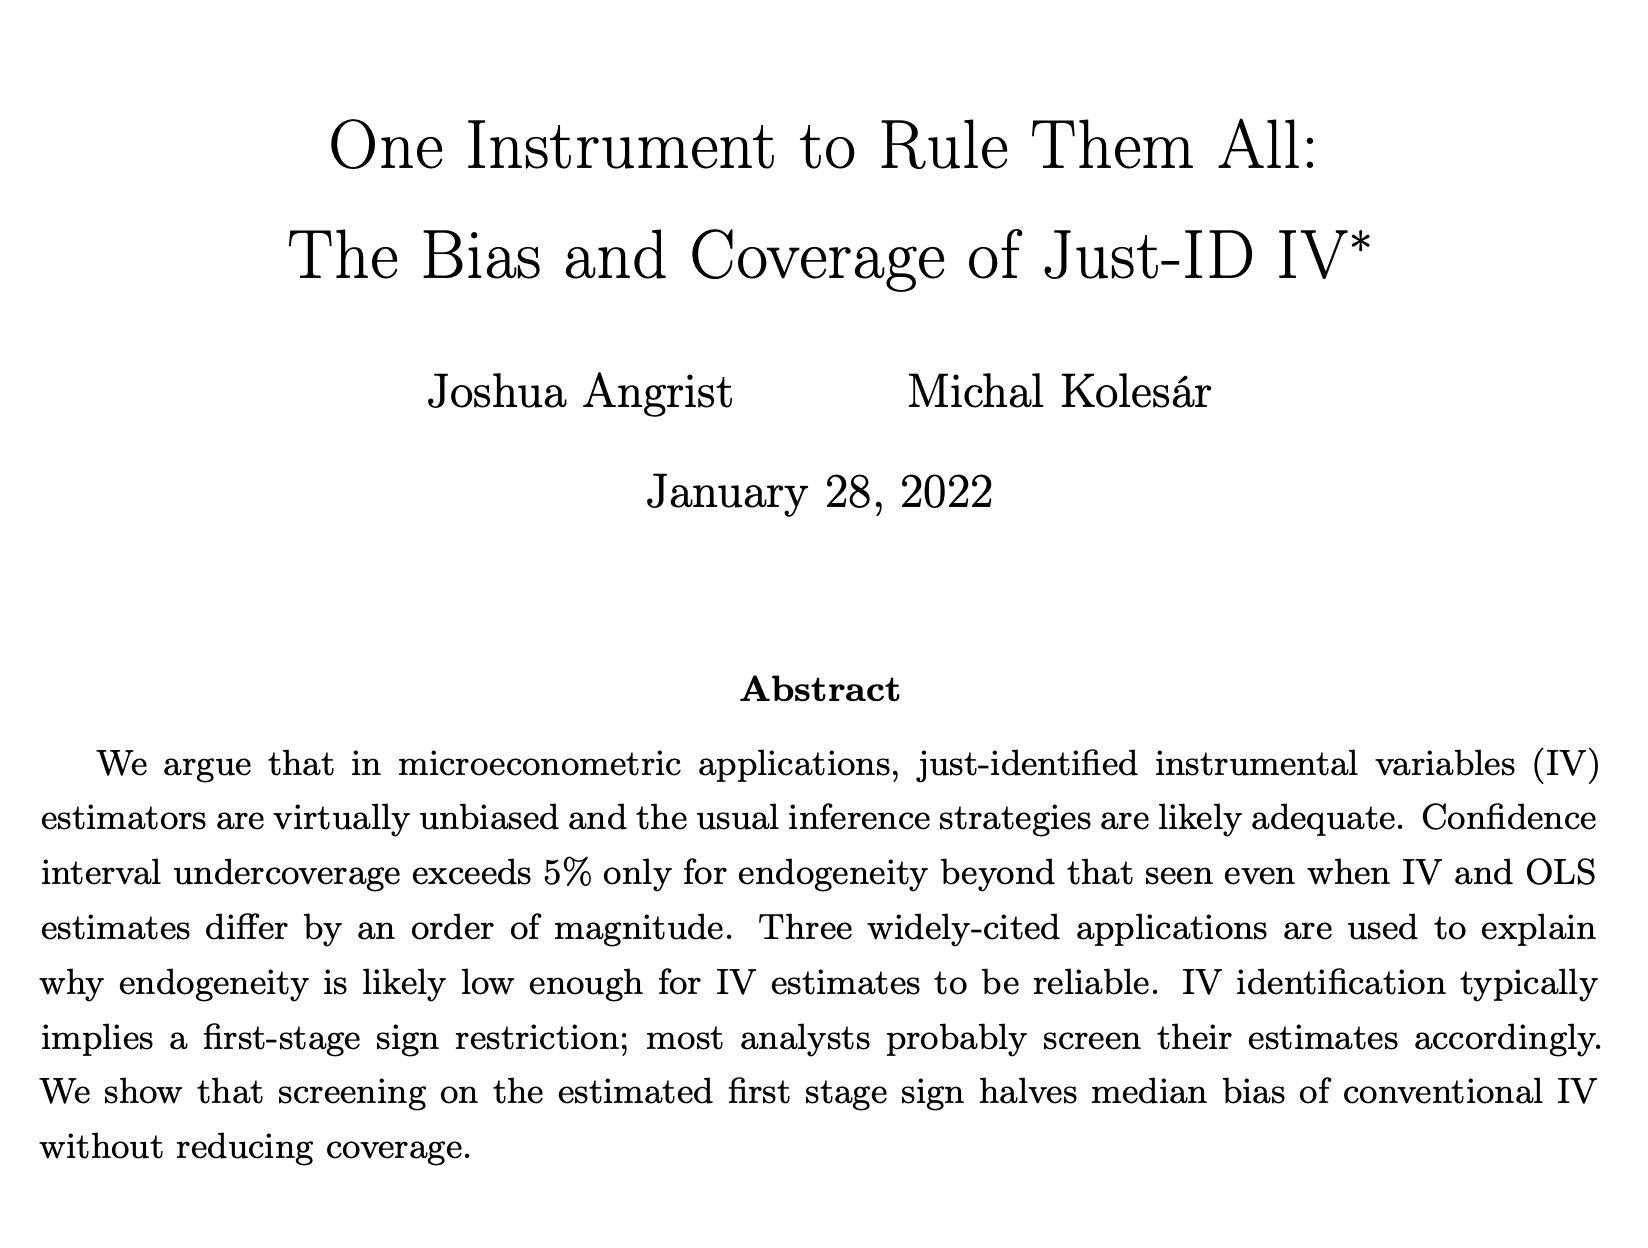
\includegraphics[width=\linewidth]{images/weakiv_kolesarangrist.png}
    \end{column}
  \end{columns}
\end{frame}


\begin{frame}{Solution 1: Pretesting}
  \begin{columns}[T] % align columns
    \begin{column}{0.5\textwidth}
      \begin{wideitemize}
      \item The arms race continues (again!). Angirst and Kolesar
        (2022) argue that weak instruments are generally \emph{not} a
        concern in the just identified case
      \item Why? How to reconcile with Lee?
        \item Punchline: endogeneity has to be \emph{extremely} high for the bias to outweigh the increase in noise
      \end{wideitemize}
    \end{column}
    \begin{column}{0.5\textwidth}
      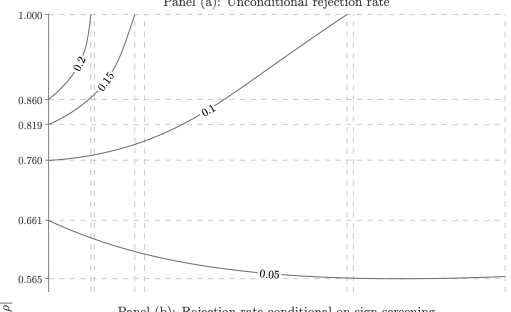
\includegraphics[width=\linewidth]{images/angristkolesar_contour.png}
    \end{column}
  \end{columns}
\end{frame}


\begin{frame}{Weak IV sims (courtesy of Peter Hull)}
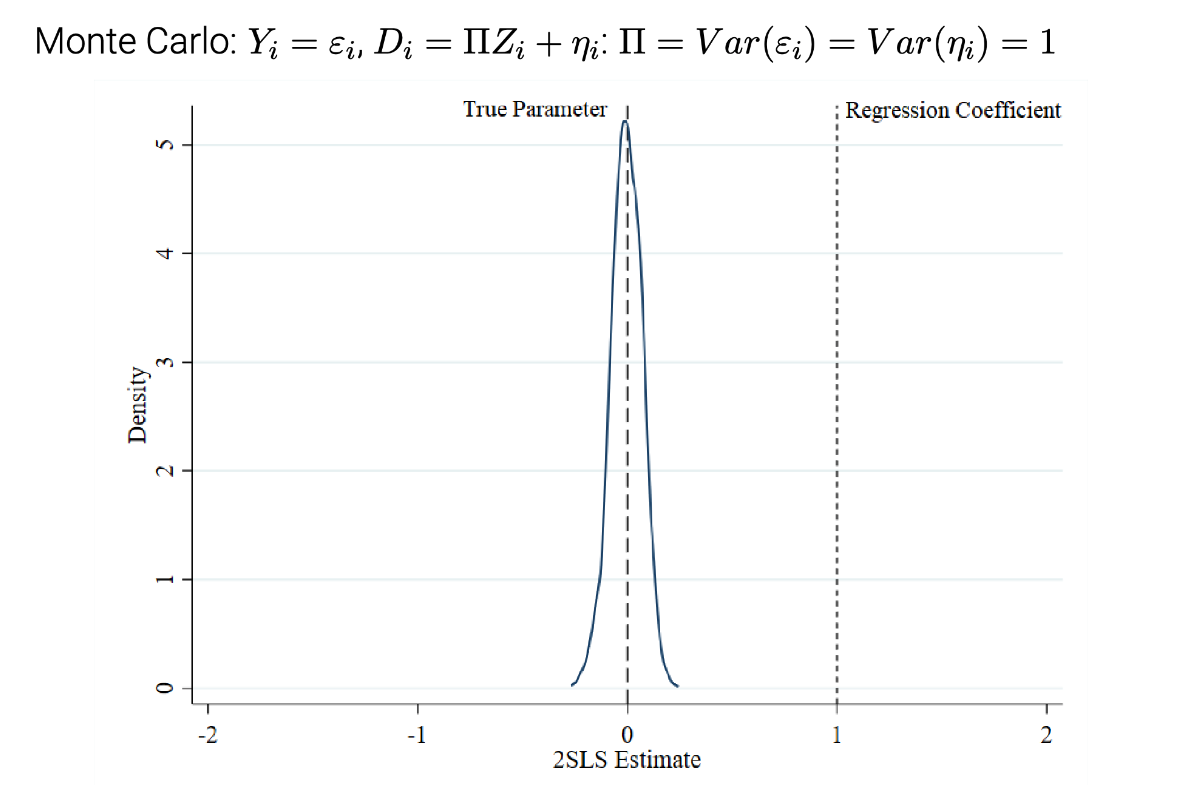
\includegraphics[width=0.7\linewidth]{images/weakiv_hull1.png}
\end{frame}
\begin{frame}{Weak IV sims (courtesy of Peter Hull)}
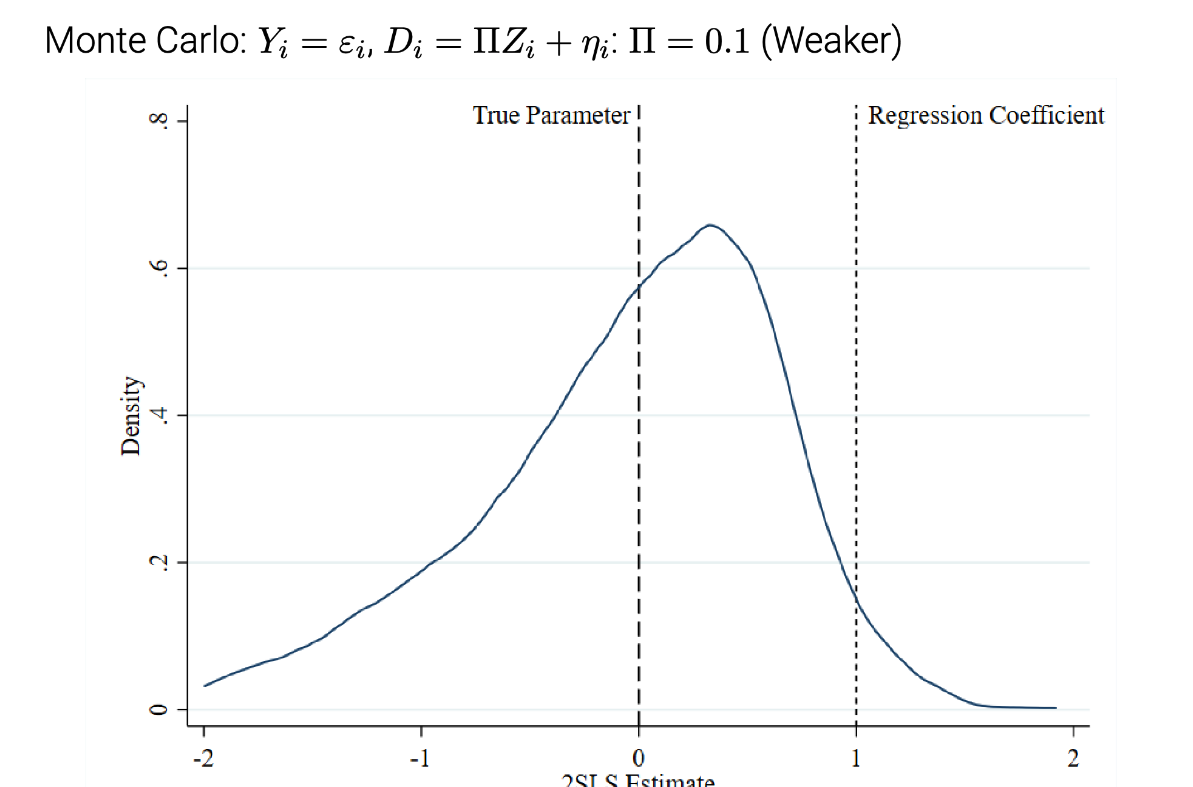
\includegraphics[width=0.7\linewidth]{images/weakiv_hull2.png}
\end{frame}
\begin{frame}{Weak IV sims (courtesy of Peter Hull)}
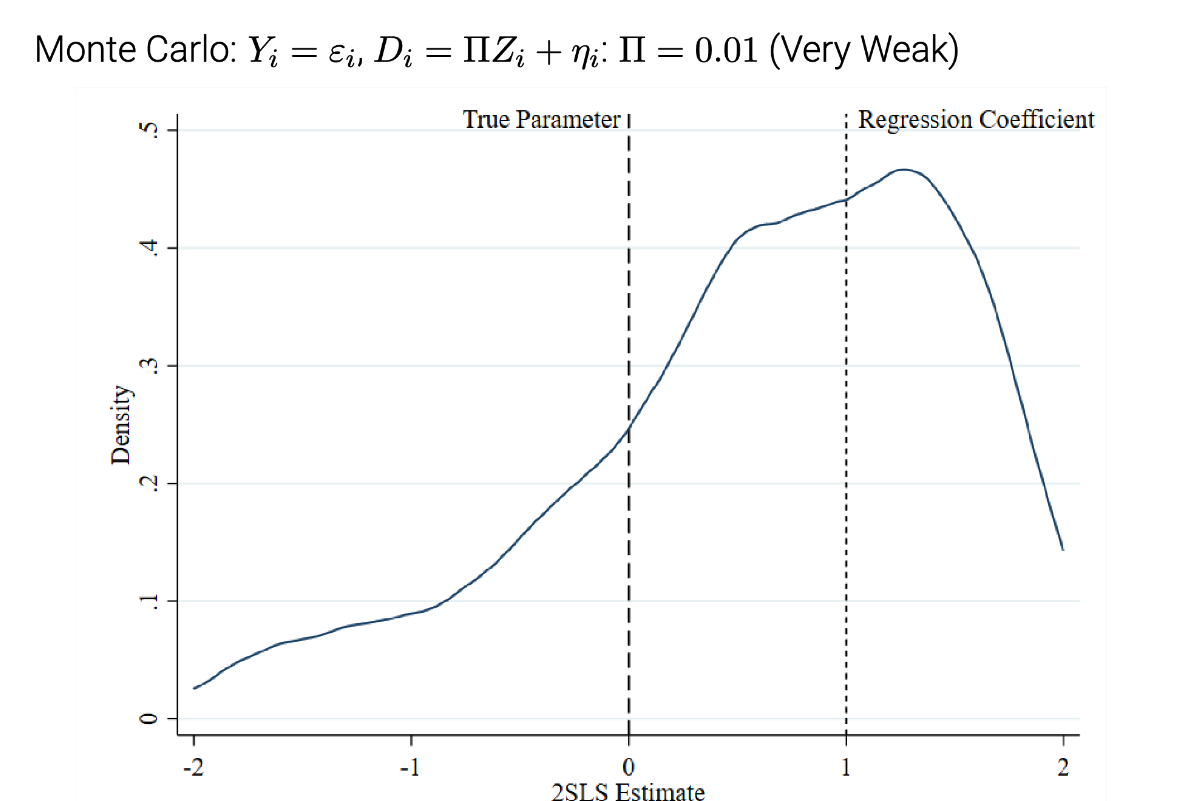
\includegraphics[width=0.7\linewidth]{images/weakiv_hull3.png}
\end{frame}

\begin{frame}{Solution 2: Robust confidence intervals}
  \begin{columns}[T] % align columns
    \begin{column}{0.5\textwidth}
      \begin{wideitemize}
      \item With a just-identified single endogeneous regressor,
        Anderson-Rubin confidence intervals are valid, irrespective of
        the weakness of the first stage
      \item This is the easiest way to deal with this inference
        problem! These results are robust regardless of your first
        stage
        \begin{itemize}
        \item Chernozhukov and Hansen (2008) discuss a very easy and simple way to implement these confidence intervals
        \item Stata and R packages are also available
        \end{itemize}
      \end{wideitemize}
    \end{column}
    \begin{column}{0.5\textwidth}
      \only<1>{\includegraphics[width=\linewidth]{images/chernhansen_weakivb.png}}
      \only<2>{\includegraphics[width=\linewidth]{images/chernhansen_weakiv.png}}      
    \end{column}
  \end{columns}
\end{frame}


\begin{frame}{Many instruments}
  \begin{columns}[T] % align columns
    \begin{column}{0.8\textwidth}
      \begin{wideitemize}
      \item Recall from our discussion above that even many instruments creates bias:
    \begin{align*}
      E(\hat{\beta}_{2SLS} - \beta) &\approx \underbrace{\frac{\sigma_{u\epsilon}}{\sigma^{2}_{u}}}_{\text{OVB}}\left[\underbrace{\frac{E(\pi'Z'Z\pi)/K}{\sigma^{2}_{u}}}_{\text{First Stage  F statistic}} + 1\right]^{-1}
    \end{align*}
  \item This is due to ``overfitting'' in the projection of 2SLS
  \item This is very solveable. Use of jackknife IV (which leaves out
    the own observation) will address this issue
    \begin{itemize}
    \item See Angrist, Imbens and Krueger (1999) for details
    \item Inference methods in this setting are a little less well-developed, however
    \end{itemize}
  \item We will revisit this issue when considering Judge IV settings
      \end{wideitemize}
    \end{column}
    \begin{column}{0.5\textwidth}
    \end{column}
  \end{columns}
\end{frame}




\end{document}


